\documentclass[UTF8,a4paper]{article}
\usepackage{ctex}
\usepackage{amsmath}
\usepackage{amssymb}
\usepackage{graphicx}
\usepackage{fancyhdr}
\usepackage{CJK}
\usepackage{chngpage}
\usepackage{url}
\setCJKmainfont{宋体}
\usepackage{listings}
\usepackage{xcolor}
\usepackage[numbers,sort&compress]{natbib}
\usepackage{xpatch}
\usepackage{geometry}
\xpatchcmd{\thebibliography}{\section*}{\section}{}{}
\geometry{left=2.9cm,right=2.9cm,top=3cm,bottom=2.9cm}

\definecolor{CPPLight}  {HTML} {686868}
\definecolor{CPPSteel}  {HTML} {888888}
\definecolor{CPPDark}   {HTML} {262626}
\definecolor{CPPBlue}   {HTML} {4172A3}
\definecolor{CPPGreen}  {HTML} {487818}
\definecolor{CPPBrown}  {HTML} {A07040}
\definecolor{CPPRed}    {HTML} {AD4D3A}
\definecolor{CPPViolet} {HTML} {7040A0}
\definecolor{CPPGray}  {HTML} {B8B8B8}


\lstset{
	columns=fixed,       
	numbers=left,                                        % 在左侧显示行号
	frame=none,                                          % 不显示背景边框
	backgroundcolor=\color[RGB]{245,245,244},            % 设定背景颜色
	keywordstyle=\color[RGB]{40,40,255},                 % 设定关键字颜色
	numberstyle=\footnotesize\color{darkgray},           % 设定行号格式
	commentstyle=\it\color[RGB]{0,96,96},                % 设置代码注释的格式
	basicstyle=\small,
	stringstyle=\rmfamily\slshape\color[RGB]{128,0,0},   % 设置字符串格式
	showstringspaces=false,                              % 不显示字符串中的空格
	language=c++,                                        % 设置语言
	morekeywords={alignas,continute,friend,register,true,alignof,decltype,goto,
		reinterpret_cast,try,asm,defult,if,return,typedef,auto,delete,inline,short,
		typeid,bool,do,int,signed,typename,break,double,long,sizeof,union,case,
		dynamic_cast,mutable,static,unsigned,catch,else,namespace,static_assert,using,
		char,enum,new,static_cast,virtual,char16_t,char32_t,explict,noexcept,struct,
		void,export,nullptr,switch,volatile,class,extern,operator,template,wchar_t,
		const,false,private,this,while,constexpr,float,protected,thread_local,
		const_cast,for,public,throw,std},
	emph={map,set,multimap,multiset,unordered_map,unordered_set,
		unordered_multiset,unordered_multimap,vector,string,list,deque,
		array,stack,forwared_list,iostream,memory,shared_ptr,unique_ptr,
		random,bitset,ostream,istream,cout,cin,endl,move,default_random_engine,
		uniform_int_distribution,iterator,algorithm,functional,bing,numeric,},
	emphstyle=\color{CPPViolet}, 
}



%opening
\title{实验一 古典密码算法及攻击方法}
\author{}
\date{}
\begin{document}

\maketitle

\begin{abstract}
通过C++编程实现移位密码和单表置换密码算法,加深对经典密码体制的了解。并通过对这两种密码实施攻击,了解对古典密码体制的攻击方法。\par 
\end{abstract}
\tableofcontents
\newpage
\section{流程图}
整体流程图如下:\par 
		\begin{center}
	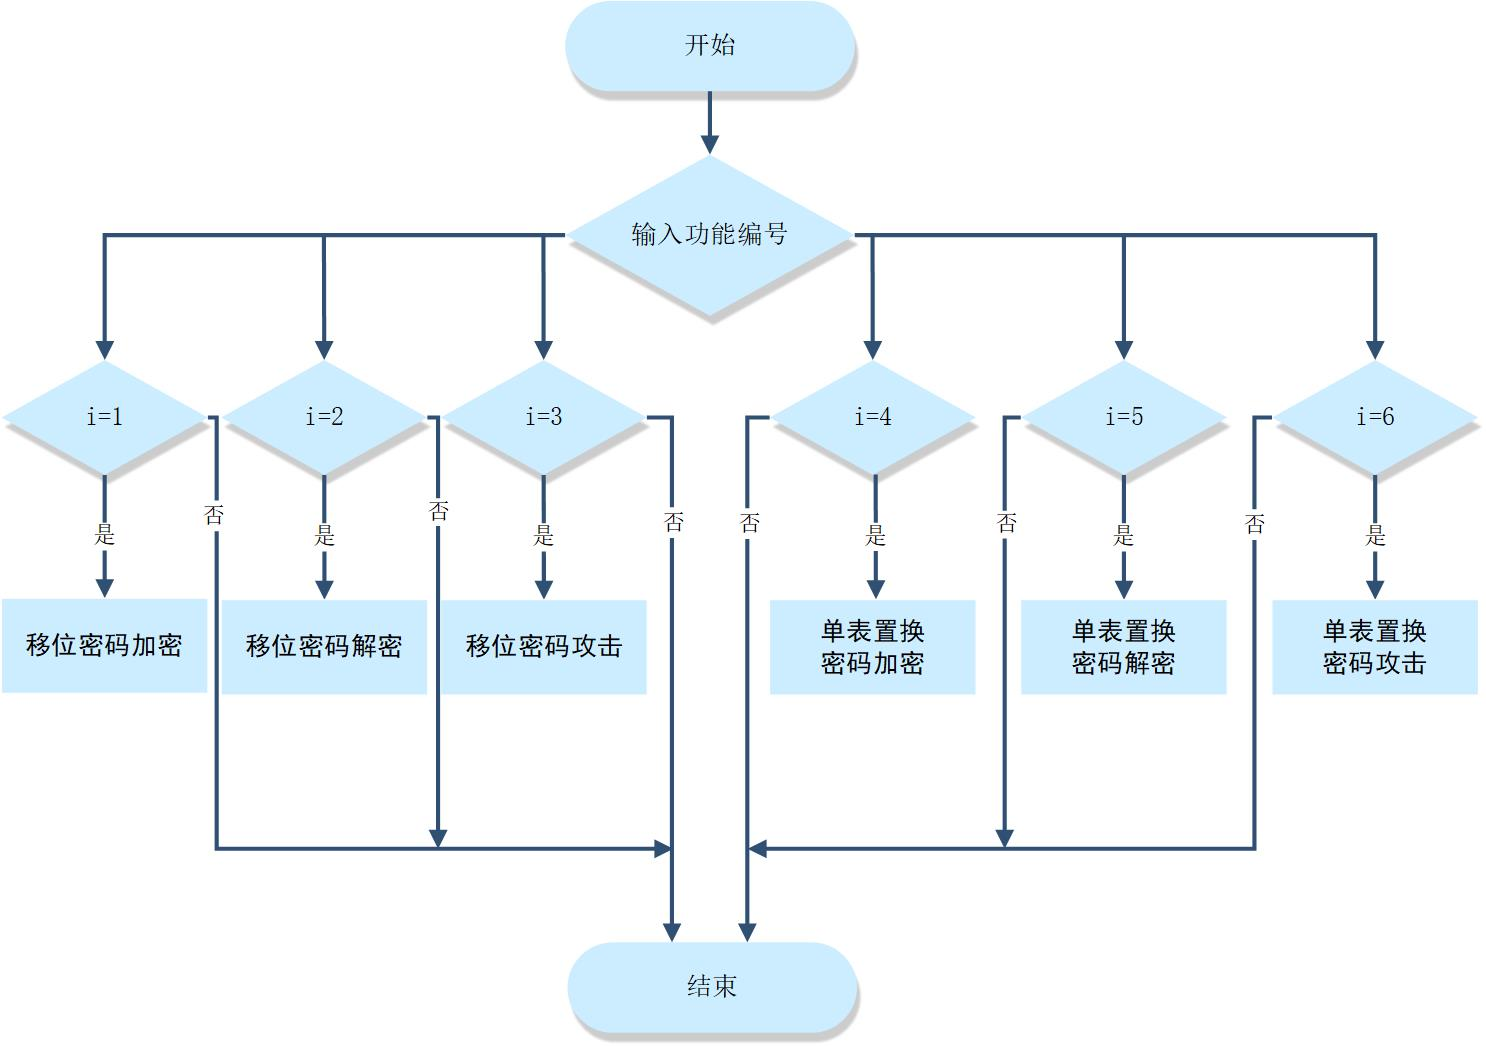
\includegraphics[width=0.9\textwidth]{all.JPG}
\end{center}
\section{移位密码}

	\subsection{实验原理}
	移位密码:将英文字母向前或向后移动一个固定位置。例如向后移动3个位
	置,即对字母表作置换(不分大小写)。\par 
	\begin{center}
	A  B  C  D  E  F  G  H  I  J  K  L  M  N  O  P  Q  R  S  T  U  V  W  X  Y  Z\par 
	D  E  F  G  H  I  J  K  L  M  N  O  P  Q  R  S  T  U  V  W  X  Y  Z  A  B  C\par 
	\end{center}

	设明文为:public keys,则经过以上置换就变成了:sxeolf nhbv。
	如果将26个英文字母进行编码:A→0,B→1,…,Z→25,则以上加密过程可简单地写成:\par 
	明文:m=$m_1$$m_2$…$m_i$…, 则有\par 
	密文:c=$c_1$$c_2$…$c_i$…, 其中 $c_i$=($m_i$+key mod26),i=1,2,…。\par 
	

	\subsection{算法流程图}
	移位密码流程图如下:\par 
	\newpage
		\begin{center}
	
		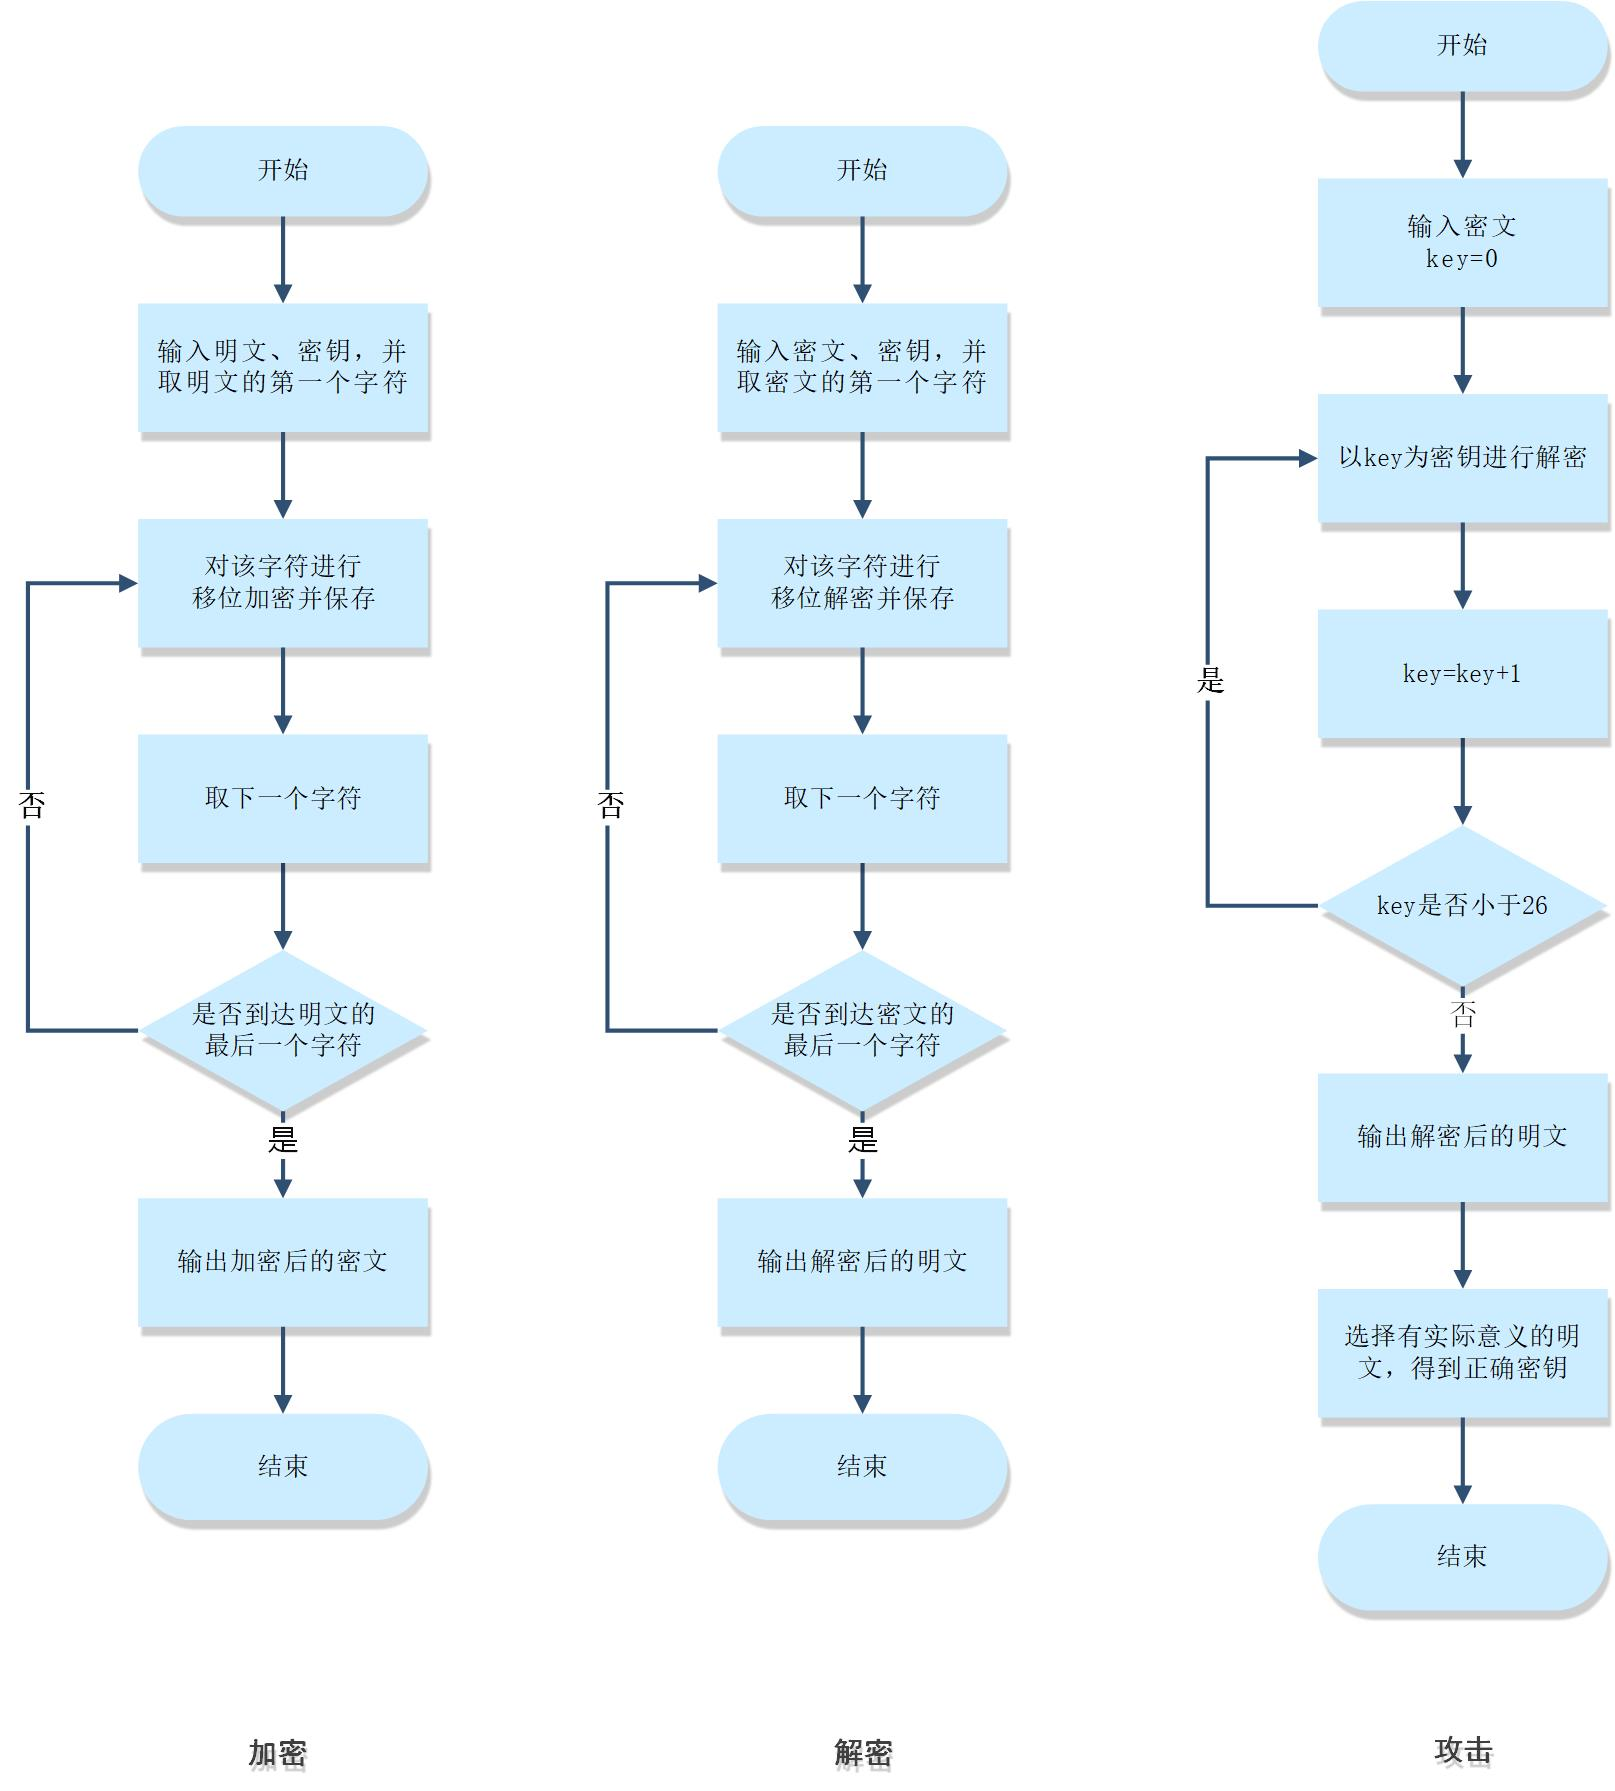
\includegraphics[width=0.86\textwidth]{first.JPG}
	\end{center}

	\subsection{移位密码攻击}
	移位密码是一种最简单的密码,其有效密钥空间大小为25。因此,很容易用穷举的方法攻破。穷举密钥攻击是指攻击者对可能的密钥的穷举,也就是用所有可能的密钥解密密文,直到得到有意义的明文,由此确定出正确的密钥和明文的攻击方法。对移位密码进行穷举密钥攻击,最多只要试译25次就可以得到正确的密钥和明文。\par 


	\subsection{实验结果}
	(一)移位密码加密:\par 

\begin{center}		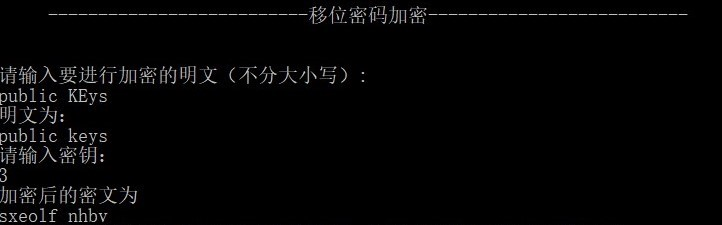
\includegraphics[width=0.6\textwidth]{firstEncry.JPG}
\end{center}

		(二)移位密码解密:\par 
\begin{center}
		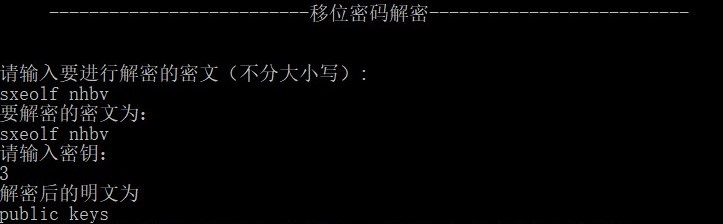
\includegraphics[width=0.6\textwidth]{firstDecry.JPG}
\end{center}

	(三)移位密码攻击:\par 

\begin{center}	
	\includegraphics[width=0.6\textwidth]{firstAttack.JPG}
\end{center}

\section{单表置换密码}

	\subsection{实验原理}
		单表置换密码就是根据字母表的置换对明文进行变换的方法,例如,给定置换:\par 
	\begin{center}
	A  B  C  D  E  F  G  H  I  J  K  L  M  N  O  P  Q  R  S  T  U  V  W  X  Y  Z\par 
	H  K  W  T  X  Y  S  G  B  P  Q  E  J  A  Z  M  L  N  O  F  C  I  D  V  U  R\par 
	\end{center}\par 
	明文:public keys, 则有密文:mckebw qxuo。\par 
	单表置换实现的一个关键问题是关于置换表的构造。置换表的构造可以有各种不同的途径,主要考虑的是记忆的方便。如使用一个短语或句子,删去其中的重复部分,作为置换表的前面的部分,然后把没有用到的字母按字母表的顺序依次放入置换表中。\par 

	\subsection{算法流程图}
	\newpage
	
		\begin{figure}[!ht]
	
	\centering
	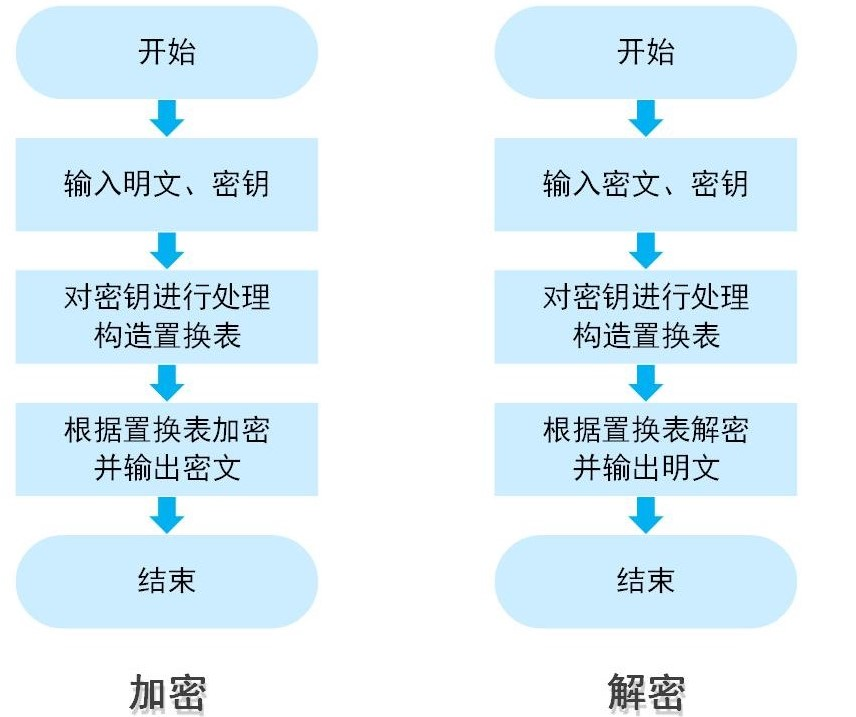
\includegraphics[width=0.55\textwidth]{second.JPG}
	\caption{单表置换密码流程图}
	\label{fig:second}
\end{figure}
		\begin{figure}[!ht]
	
	\centering
	
\includegraphics[width=1.1\textwidth]{getkey.JPG}
	\caption{置换表构造}
	\label{fig:getkey}
\end{figure}


		\begin{figure}[!ht]
	
	\centering
	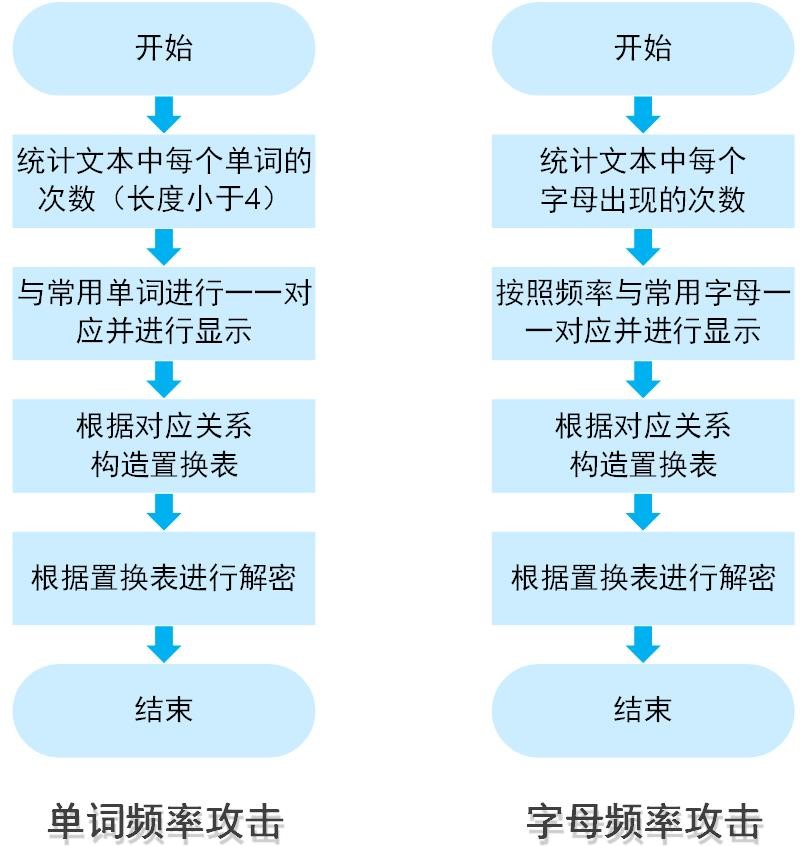
\includegraphics[width=0.55\textwidth]{secondAttack.JPG}
	\caption{单表置换密码攻击流程图}
	\label{fig:secondAttack}
\end{figure}



	\subsection{单表置换密码攻击}
	在单表置换密码中,由于置换表字母组合方式有26!种,约为4.03×$10^{26}$。\par 
	所以采用穷举密钥的方法不是一种最有效的方法。对单表置换密码最有效的攻击方法是利用自然语言的使用频率:单字母、双字母组/三字母组、短语、词头/词尾等,这里仅考虑英文的情况。英文的一些显著特征如下:\par 
	短单词(small words):在英文中只有很少几个非常短的单词。因此,如果在一个加密的文本中可以确定单词的范围,那么就能得出明显的结果。一个字母的单词只有a和I。如果不计单词的缩写,在从电子邮件中选取500k字节的样本中,只有两个字母的单词仅出现35次,而两个字母的所有组合为26×26=676种。而且,还是在那个样本中,只有三个字母的单词出现196次,而三个字母的所有组合为26×26×26=17576种。\par 
	常用单词(common words):再次分析500k字节的样本,总共有5000多个不同的单词出现。在这里,9个最常用的单词出现的总次数占总单词数的21%,20个最常用的单词出现的总次数占总单词数的30%,104个最常用的单词占50%,247个最常用的单词占60%。样本中最常用的9个单词占总词数的百分比为:\par 
	\begin{center}
	the-4.65   \qquad   to-3.02   \qquad  of-2.61 \qquad   I-2.2   \qquad a-1.95\qquad \par 
	and-1.82    \qquad  is-1.68  \qquad   that-1.62 \qquad   in-1.57
\end{center}\par 
	字母频率(character frequency):在1M字节旧的电子文本中,对字母”A”到“Z”(忽略大小写)分别进行统计。发现近似频率(以百分比表示):\par 
		\begin{center}
	e-11.67  \qquad  t-9.53  \qquad  o-8.22 \qquad   i-7.81 \qquad    a-7.73  \qquad  n-6.71 \qquad  s-6.55 
	r-5.97 \qquad    h-4.52  \qquad  l-4.3  \qquad   d-3.24  \qquad  u-3.21  \qquad  c-3.06  m-2.8
	p-2.34  \qquad   y-2.22 \qquad   f-2.14 \qquad   g-2.00 \qquad   w-1.69  \qquad  b-1.58\qquad   v-1.03
	k-0.79  \qquad   x-0.30   \qquad j-0.23\qquad    q-0.12  \qquad  z-0.09
\end{center}\par 
	从该表中可以看出,最常用的单字母英文是e和t,其他字母使用频率相对来说就小得多。这样,攻击一个单表置换密码,首先统计密文中最常出现的字母,并据此猜出两个最常用的字母,并根据英文统计的其他特征(如字母组合等)进行试译。\par 
	

	\subsection{实验结果}
	
		(一)移位密码加密:\par 
	
	\begin{center}		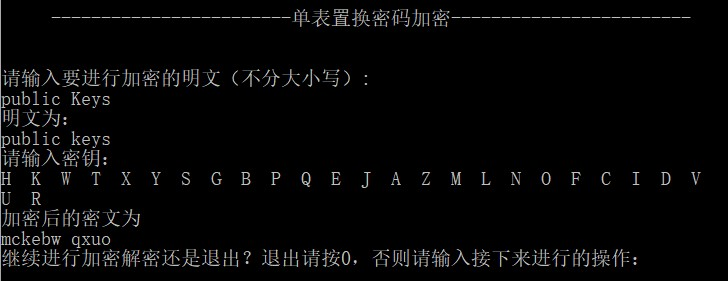
\includegraphics[width=0.6\textwidth]{secondEncry.JPG}
	\end{center}
	
	(二)移位密码解密:\par 
	\begin{center}
		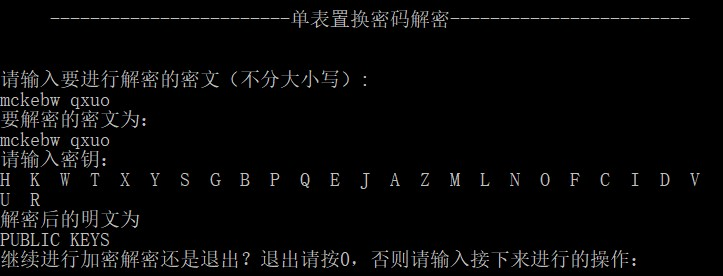
\includegraphics[width=0.6\textwidth]{secondDecry.JPG}
	\end{center}
	
	(三)移位密码攻击:\par 
	1.单词频率攻击:\par 
		\begin{center}
		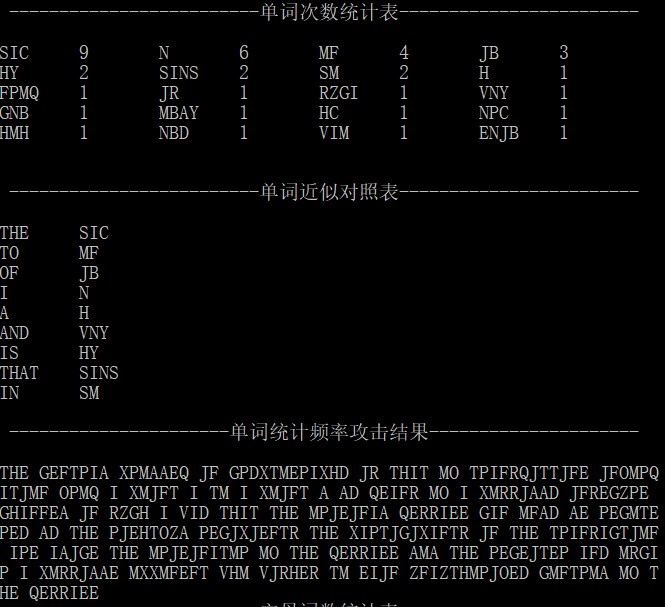
\includegraphics[width=0.6\textwidth]{2attack1.JPG}
	\end{center}


	2.字母频率攻击:\par 
			\begin{center}
		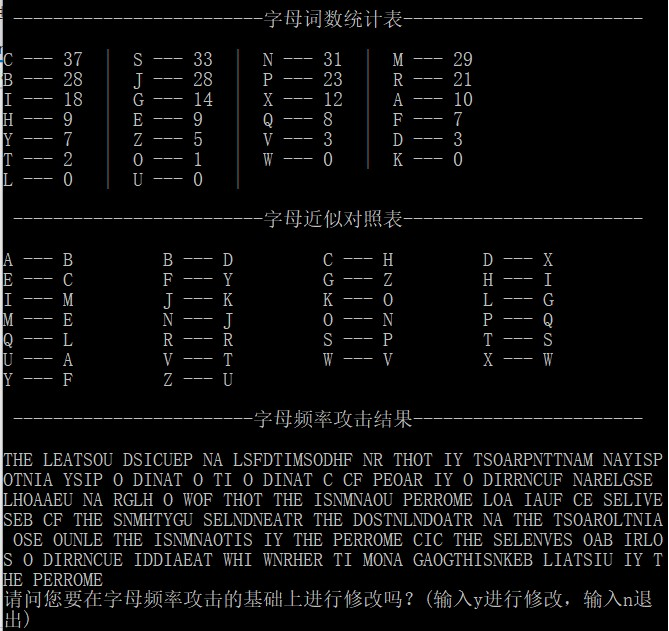
\includegraphics[width=0.6\textwidth]{2attack2.JPG}
	\end{center}

	3.在字母频率攻击的基础上继续攻击:\par 
	(1)观察到明文中的第一行出现了thot一词,依据常用单词,将其修改为that。
				\begin{center}
		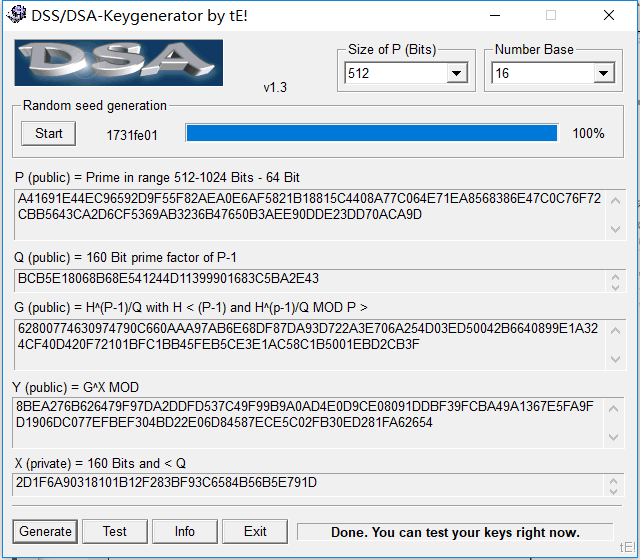
\includegraphics[width=0.6\textwidth]{pic1.JPG}
	\end{center}

	(2)观察到明文中的第一行出现了iy一词,依据常用单词,将其修改为of。\par 
					\begin{center}
		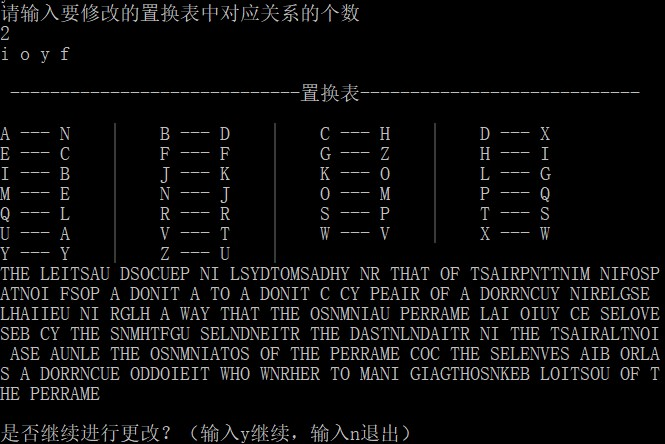
\includegraphics[width=0.6\textwidth]{pic2.JPG}
	\end{center}

	(3)此时明文中多次出现以n开头的双字幕段单词,推测其为is,所以将nr改为is。\par 
					\begin{center}
		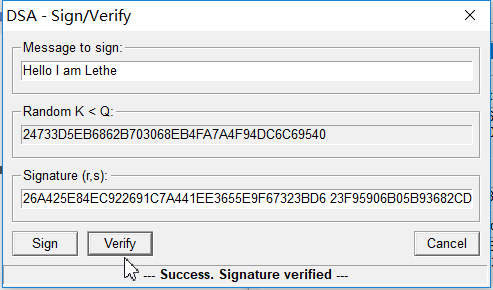
\includegraphics[width=0.6\textwidth]{pic3.JPG}
	\end{center}

	(4)发现现在的明文中有frop,推测其为from,因此,将p换为m。\par 
					\begin{center}
		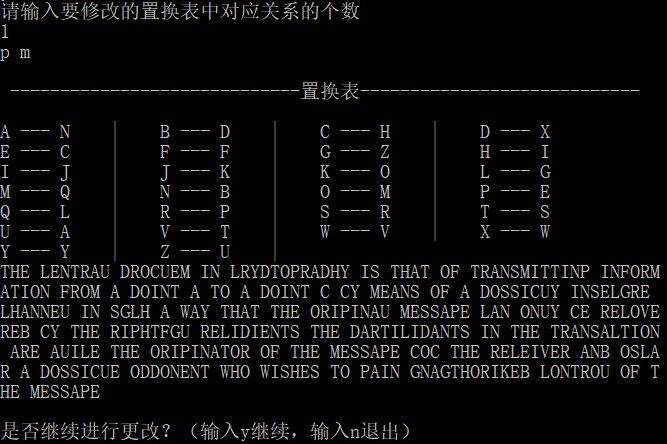
\includegraphics[width=0.6\textwidth]{pic4.JPG}
	\end{center}

	(5)发现doint一词,根据常用单词将其修改为point。\par 
					\begin{center}
		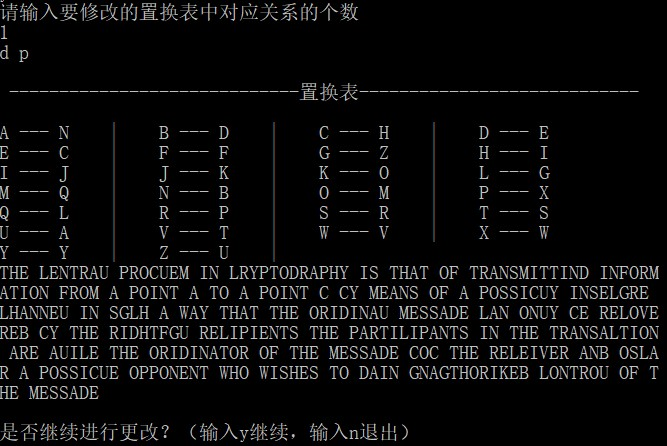
\includegraphics[width=0.6\textwidth]{pic5.JPG}
	\end{center}

	(6)根据“from a point a to a point c”和cy,推测应该将c换成b。\par 
					\begin{center}
		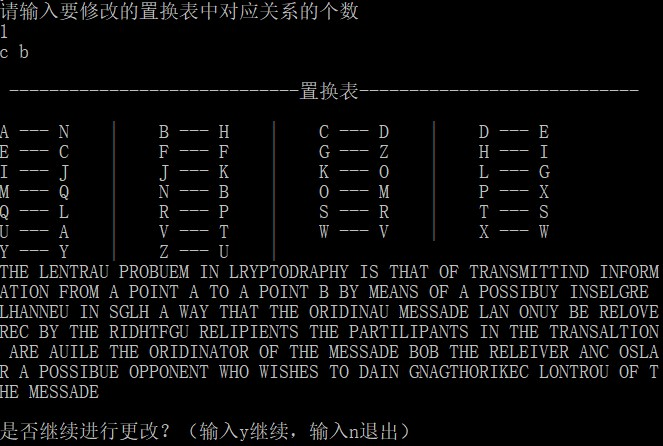
\includegraphics[width=0.6\textwidth]{pic6.JPG}
	\end{center}

	(7)存在单词probuem,推测其为problem,所以将u换成l。\par
	(8)存在单词uentral,推测其为central,所以将u换成c。\par
	(9)存在单词cryptodraphy,推测其为crytography,所以将d换成g。\par
	(10)存在单词insecdre,推测其为insecure,所以将d换成u。\par
	(11)存在单词unauthoriked,推测其为unauthorized,所以将k换成z。\par
	(12)最后结果如下:\par
						\begin{center}
		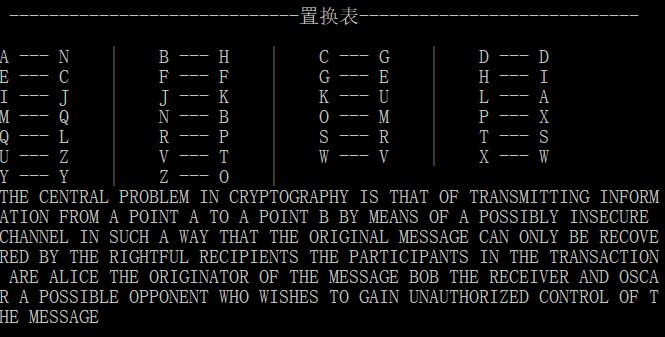
\includegraphics[width=0.6\textwidth]{pic.JPG}
	\end{center}

\end{document}
